\documentclass[12pt, english, twoside]{article} %twoside necessary for fancyheader odd vs. even commands 

\usepackage[letterpaper]{geometry}
%\geometry{verbose, a4paper, tmargin=1in,bmargin=1in,lmargin=1.25in,rmargin=1.25in}
\geometry{verbose, a4paper, tmargin=3cm,bmargin=3cm,lmargin=3cm,rmargin=3cm} 

\usepackage{amsmath, hyperref, enumerate, comment}
\usepackage{amsfonts, esint, setspace}
\usepackage{graphicx}
\usepackage{mathrsfs} %for script font 

\linespread{1.3}	

\raggedbottom % prevents random spaces between paragraphs from appearing

\usepackage[titletoc,title]{appendix}

% headers
\usepackage{fancyhdr} 
\pagestyle{fancy}
\fancyhead{}
\fancyhead[OR,ER]{\large \textbf{\thepage}}
%\fancyhead[C]{\textit{}}% odd page header and number to right top
%\fancyhead[EC]{\textit{Your Name}}%Even page header and number at left top
\fancyfoot[L,R,C]{}
\renewcommand{\headrulewidth}{0pt}
%\renewcommand{\footrulewidth}{0pt}
\renewcommand*\footnoterule{} %removes footnote line


% % redefines abstract to be capitalized, with no margins 
\renewenvironment{abstract}
 {\small
  \begin{center}
\normalsize  \textnormal{ABSTRACT\\} \vspace{-0em}\vspace{0pt}
  \end{center}
  \list{}{%
    \setlength{\leftmargin}{0in}%
    \setlength{\rightmargin}{\leftmargin}%
  }%
  \item\relax}
 {\endlist}

% section headings
\usepackage{sectsty}
\allsectionsfont{\large\raggedright\centering}

% Table of contents stuff and footnotes 
\setcounter{tocdepth}{2}
\usepackage[]{tocloft}
%\addtocontents{toc}{\cftpagenumbersoff{section}} % turns off page numbers from section level 
%\addtocontents{toc}{\cftpagenumbersoff{subsection}} %like wise for subsection level 
\renewcommand{\cftsecfont}{\itshape}
\renewcommand{\cftsubsecfont}{\itshape}
\renewcommand{\cftsecpresnum}{\normalfont \bfseries} % puts the section numbers in non-italics and bold
\renewcommand{\cftsubsecpresnum}{\normalfont \bfseries} % likewise for subsection numbers 

\renewcommand{\cftbeforesecskip}{3pt} %controls spacing between ToC items 
\makeatletter
\renewcommand{\@cftmaketoctitle}{}

% % footnote modification: must be between \makeatletter and \makeatother

\renewcommand{\@makefntext}[1]{%
  \setlength{\parindent}{0pt}%
  \begin{list}{}{\setlength{\labelwidth}{6mm}% indents footnote text 
    \setlength{\leftmargin}{\labelwidth}%
    \setlength{\labelsep}{5pt}% moves footnote mark to the left
     \setlength{\itemsep}{0pt}%
      \setlength{\parsep}{0pt}%
      \setlength{\topsep}{-3pt}% removes separation between footnotes
    \footnotesize}%
  \item[\@textsuperscript{\@thefnmark}\hfil ]#1% @makefnmark
  \end{list}%
}
%      \setlength{\footnotesep}{0pt}%

\makeatother
\renewcommand{\cftdot}{} % removes dots from table of contents 


% % for fonts:
\usepackage[T1]{fontenc}
\usepackage[utf8]{inputenc}
\usepackage{mathptmx}

% Hyperref set-up & metadata
\hypersetup{
	pdftitle={Your Paper Title},
	pdfauthor={Your Name},
	pdfsubject={},
	pdfkeywords={},
	pdfcreator={XeLaTeX},
	pdfproducer={XeLaTeX},
	pdftoolbar=false,	% show Acrobat’s toolbar?
	pdfmenubar=true,	% show Acrobat’s menu?
	pdffitwindow=false,	% window fit to page when opened
	pdfstartview={FitH},	% fits the width of the page to the window
	unicode=true,		% non-Latin characters in Acrobat’s bookmarks
	pdfnewwindow=true,	% links in new window
	colorlinks=true,	% false: boxed links; true: colored links
	linkcolor=black,	% color of internal links
	citecolor=black,	% color of links to bibliography
	filecolor=black,	% color of file links
	urlcolor=blue		% color of external links
}


%\usepackage[backend=biber, style=authoryear, url=false, doi=false, eprint=false]{biblatex}




% % % Biblatex commands for Citations and References:
\usepackage[backend=biber, style=ext-authoryear-comp,  maxcitenames=2, dashed=false, url=false, doi=false, eprint=true, giveninits=true, innamebeforetitle=true, maxbibnames=6]{biblatex} 

\addbibresource{bibliography.bib}

%\addbibresource{templateReferences.bib} %%generated by reference items above
%maxcitenames=2 replaces all instances of more than 2 authors in citations with `et al.', but lists all authors in references
%labeltitleyear=true; sortcites=true
%innamebeforetitle=true places editors before the book titles
%style=authoryear-comp adds in some weird ``In:'' stuff in reference list that must be changed below. 

\DeclareFieldFormat{labeldate}{\mkbibbrackets{#1}} %puts brackets around years in citations

\DeclareFieldFormat{postnote}{\mkpageprefix[pagination][\mkcomprange]{#1}} % compresses page range in citations, so that unchanged digits are not repeated. See p. 259, section 4.6.4 of biblatex manual.  %also adds pagination prefix p.

% clears un-needed fields from reference items
\AtEveryBibitem{%
 \clearfield{note}%
  \clearfield{series}%
 \clearfield{number}%
 \clearfield{pagetotal}%
 \clearfield{chapter}%
  }
  %\clearfield{pages}%}
  
  
  \renewcommand{\newunitpunct}{\addcomma\space} %makes a comma the default separator between items; overridden in some cases by commands below

\renewcommand{\intitlepunct}{\addspace\nopunct} %removes punctuation after ``in"

\DeclareDelimFormat[bib,biblist]{nametitledelim}{\addcolon\space} %puts colon after year

\DeclareFieldFormat{biblabeldate}{\mkbibbrackets{#1}} %puts brackets around years in references

\DeclareFieldFormat{editortype}{\mkbibparens{\textit{#1}}} %puts ed in parentheses
\DeclareDelimFormat{editortypedelim}{\addspace}%prevents punctuaction clash after (ed)
\DeclareDelimFormat[bib,biblist]{innametitledelim}{\addcomma\space} % puts comma after (ed)

\DeclareFieldFormat{eprint}{\printtext{available at}\addspace \textless#1\textgreater} % Calls url from Eprint field. See biblatex manual, section 4.11.2 Electronic Publishing Information, page 310-11
  
\DeclareFieldFormat[article,periodical]{volume}{\textbf{#1}} %puts volume in bold; note that adding \bibstring{jourvol}~ before #1} prints ``vol.". from biblatex-ext manual 
%\DeclareFieldFormat[article,periodical]{number}{#1}%\bibstring{number}~ before #1} prints ``vol."
\renewcommand*{\jourvoldelim}{\addcomma\space} %combined with above command, puts comma after article title and before journal volume. 
%\renewcommand*{\volnumdelim}{\addcomma\space}

\DeclareFieldFormat[inbook, incollection, book]{volume}{\bibcpstring{volume}~#1} %capitalizes `Vol' after book titles. 

\DeclareFieldFormat{pages}{\mkpageprefix[pagination][\mkcomprange]{#1}} % compresses page range in bibliography, so that unchanged digits are not repeated. 

% % following command suppresses ``in" for articles and inproceedings only
\renewbibmacro{in:}{%
\ifboolexpr{%
test {\ifentrytype{article}}%
or
test {\ifentrytype{inproceedings}}%
}
{}%<-nothing
{\printtext{\bibstring{in}\intitlepunct}}%<-normal ’in’ with punctuation
}


\newcommand{\diff}{\mathop{}\!\mathrm{d}} %defines exterior derivative 
\renewcommand{\div}[1]{\gv{\nabla} \cdot #1} % for divergence
\newcommand{\curl}[1]{\gv{\nabla} \times #1} % for curl
\renewcommand{\vector}[1]{\ensuremath{\vec{#1}}} % redefines vector to vec
\newcommand{\integral}{\int}

\newcommand\bs{\begin{singlespace}} 			
\newcommand\es{\end{singlespace}} 	

\begin{document}
\title{\vspace{-2em} Hamiltonian Privilege}
%\author{TBD}

\date{\vspace{-3em} \today}

\maketitle

% 300 words maximum for BJPS
\vspace{-3em}
\bs
\begin{abstract}
\noindent We argue that Hamiltonian mechanics is more fundamental than Lagrangian mechanics. Our argument provides a non-metaphysical strategy for privileging one formulation of a theory over another: a formulation is more fundamental at least when it is more general. We illustrate this criterion through a novel interpretation of classical mechanics in terms of three physical conditions. Two of these conditions suffice for recovering Hamiltonian mechanics. A third condition is necessary for recovering Lagrangian mechanics. This shows that Lagrangian systems are a proper subset of Hamiltonian systems, elucidating the connection between these two formalisms. Moreover, we argue that the invariant phase space density is physically fundamental. Since Hamiltonian mechanics provides the proper setting for this density, we gain another reason for privileging it over Lagrangian mechanics. We interpret Lagrangian mechanics within the Hamiltonian framework, providing a geometric interpretation of the principle of stationary action. Finally, we rebut arguments for privileging Lagrangian mechanics, showing where they go wrong. 
\end{abstract}
\es

\bs
\tableofcontents 
\es

\section{Introduction}
\label{introduction}


The intellectual richness of classical mechanics manifests itself in an abundance of formulations, with Newtonian, Hamiltonian, Lagrangian, and Hamilton--Jacobi being among the most prominent.  Butterfield \parencites*[]{Butterfield2004} has aptly referred to these formulations as different \textit{schemes} for treating classical systems. Recent work in philosophy of science has focused largely on how these schemes relate to one another, with the aim of arriving at a deeper understanding of classical mechanics. By considering the conceptual differences between these formulations, we can better interpret the physical significance of our representations.

In the context of comparing Hamiltonian and Lagrangian mechanics, three interpretive stances have emerged. \textcites[]{North} has argued for privileging Hamiltonian mechanics on the grounds that it requires less mathematical structure to formulate. In contrast, \textcites[]{Curiel} recommends privileging Lagrangian mechanics, arguing that it isolates physically-significant kinematical constraints that all classical systems must satisfy. Finally, we can interpret Lagrangian and Hamiltonian mechanics as theoretically equivalent in a precise mathematical sense. Within a subclass of systems known as the \textit{hyper-regular domain}, the two formalisms are categorically equivalent \parencites[]{Teh}{Barrett2}. Categorical equivalence provides a natural interpretive criterion for theoretical equivalence because it yields mutual inter-translatability between theory formulations. This equivalence motivates the view that there are no physically significant differences between these two formalisms, at least within the hyper-regular domain. 

Here, we will argue that there are indeed physical grounds for privileging Hamiltonian mechanics over Lagrangian mechanics, their categorical equivalence notwithstanding.\footnote{Barrett shows that in the hyper-regular domain, Lagrangian and Hamiltonian mechanics are categorically equivalent provided that we define categories of models over the tangent and cotangent bundle formulations, respectively \parencites*[1181-82]{Barrett2}. However, he also shows that if we consider a more general formulation of Hamiltonian mechanics on a symplectic manifold (which does not require a cotangent bundle), then the two formulations are \textit{not} categorically equivalent \parencites*[1182-83]{Barrett2}. Our construction of Hamiltonian mechanics in Section~\ref{derivation} matches this more general symplectic manifold formulation.} Whereas North's argument relies on a problematic criterion for comparing structure based on the size of symmetry groups \parencites[]{Swanson}, our argument avoids this pitfall. We show that a classical system needs to satisfy strictly fewer physical conditions in order to be Hamiltonian. To be Lagrangian, systems must satisfy an additional physical condition, making Lagrangian mechanics a proper subset of Hamiltonian mechanics. Hamiltonian mechanics thereby captures a wider range of systems than Lagrangian mechanics, and this difference has interpretive consequences even within the hyper-regular domain. The construction at the heart of our argument provides an interpretation of classical mechanical systems in terms of their invariant phase space density. We show that the invariant density fits more naturally within the Hamiltonian framework, providing another reason to privilege it over Lagrangian mechanics.
% Our formalism also provides a novel interpretation of the principle of stationary action within Hamiltonian mechanics.

Section~\ref{privileging} previews our argument for privileging Hamiltonian mechanics. We introduce three physical conditions that define classical systems while distinguishing Hamiltonian from Lagrangian mechanics. Section~\ref{fundamentality} explains how our position differs from North's. Specifically, our argument does not require metaphysical commitments to fundamental structure or perfectly natural properties. Section~\ref{derivation} describes in detail the derivation of Hamiltonian mechanics for systems that satisfy two physical conditions: infinitesimal reducibility and deterministic/reversible evolution. We then show that Lagrangian systems must satisfy an additional physical condition, which we call motion equivalence. This completes our primary argument for privileging Hamiltonian mechanics.

Subsequent sections describe additional advantages of Hamiltonian mechanics, along with further interpretive benefits of our approach. Section~\ref{density} explains how the invariant phase space density plays a special role in the Hamiltonian framework. The density allows us to compare and track the amount of matter in different regions of phase space. In contrast, Lagrangian mechanics does not support these important properties of the density. Finally, Section~\ref{Lagrangian} considers the status of Lagrangian mechanics within our framework. We provide a geometric interpretation of the action principle, which applies even outside the hyper-regular domain. We end by rebutting objections that arise from Curiel's \parencites*[]{Curiel} privileging of Lagrangian mechanics. 
%Along the way, we examine the gauge redundancy of both the conjugate momentum (Section~\ref{gauge_momentum}) and the Lagrangian (Section~\ref{gauge}).

%Despite being coordinate-invariant, one cannot make the density truly coordinate independent. We therefore argue that some quantities are physically significant despite being coordinate-dependent. 


\section{Privileging Hamiltonian mechanics}
\label{privileging}

In claiming that Hamiltonian mechanics is more fundamental than Lagrangian mechanics, we must clarify what we mean by `fundamental.' Of the various notions of fundamentality, we will mean something entirely non-mysterious: a formalism is more fundamental provided that it is logically more general. In this case, the Lagrangian framework is less general because it requires an additional condition to hold, compared to the Hamiltonian framework. Hence, the Lagrangian framework is less fundamental because it is a proper subset of the Hamiltonian framework.\footnote{One might worry that our criterion for fundamentality is subject to elementary counterexamples. For instance, can't we make any theory more general by adjoining arbitrary disjunctions? Importantly, we require that the theory remains wholly \textit{about} classical mechanics. Hamiltonian mechanics is more general than Lagrangian mechanics while still being about classical systems, where `aboutness' can be understood using Yablo's framework \parencites*[]{Yablo}. Having an account of \textit{aboutness} or \textit{subject matter} is a general philosophical problem that any account of fundamentality or essence must address. Hence, it is not a special problem facing our criterion.}

Our argument has three main steps, summarized in Figure~\ref{diagram}. The left column lists three basic physical conditions: infinitesimal reducibility, determinism/reversibility, and motion equivalence. Each condition entails physically significant properties, described in the middle column. Each physical property corresponds to a formal/mathematical structure depicted in the right column, including phase space, Hamiltonian mechanics, and Lagrangian mechanics. In this way, our framework develops a correspondence between physical conditions and their associated mathematical formalisms. We thereby gain a straightforward interpretation of the physical significance of these formalisms.

\begin{figure}[h]
	\centering
	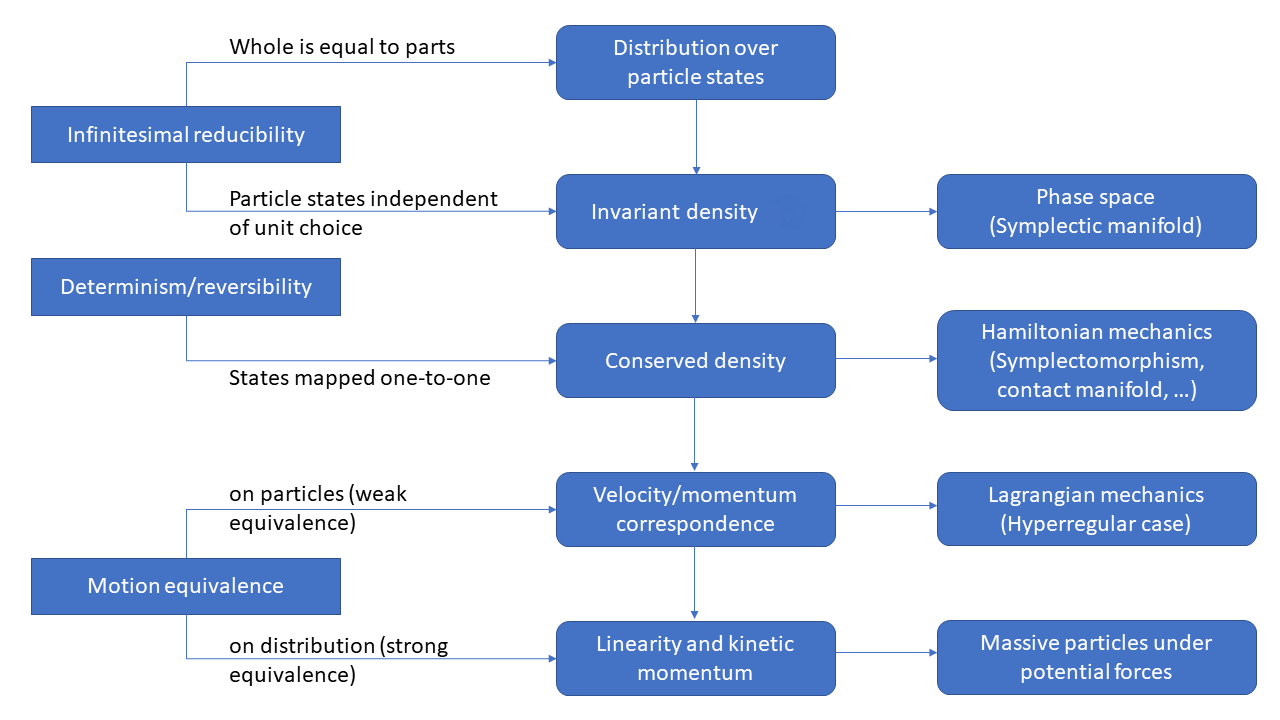
\includegraphics[width=\textwidth]{Diagram.png}
\caption{Physical conditions and corresponding properties and formalisms}
\label{diagram}
\end{figure}

First, a system is \textit{infinitesimally reducible} provided that the state of the whole system is equivalent to specifying the states of its parts (and vice versa). Infinitesimal reducibility distinguishes classical from quantum systems, where the latter are irreducible (i.e. we cannot specify the whole state by specifying the states of its subsystems). In the widest sense, a classical system is any infinitesimally reducible system. Colloquially, we can say that the whole state equals the sum of its parts, where we take these infinitesimal parts to be classical particles. 

If a system is infinitesimally reducible, then we can define a distribution $\rho$ over particle states and a density $\rho_{\xi}$ over the corresponding state variables $\xi$. Since particle states are independent of a choice of units, this density must be invariant. We show in Section~\ref{infinitesimal} that defining this invariant density requires a symplectic manifold, which serves as the phase space of classical mechanics. The physical significance of this symplectic manifold is thereby its connection with the physical condition of infinitesimal reducibility. 

Secondly, a system has \textit{deterministic and reversible evolution} provided that the present state of the system uniquely determines both its future and past states. This condition entails that the invariant density $\rho_{\xi}$ is a conserved phase space density. We will show that a classical system which satisfies this condition is Hamiltonian: its phase space is a symplectic manifold that evolves according to Hamiltonian evolution  (i.e. according to a symplectomorphism). We thereby characterize Hamiltonian mechanics as the mathematical framework for infinitesimally reducible systems with deterministic and reversible evolution. Section~\ref{deterministic} justifies this correspondence. 

Finally, some classical systems satisfy a further condition, which we call \textit{motion equivalence}. Motion equivalence holds when the system's trajectory in physical space determines---and is determined by---its evolution in phase space. In other words, knowledge of the trajectory in physical space (e.g. Euclidean three-space $\mathbb{R}^3$) suffices for knowledge of the trajectory in phase space, and vice versa. Physically, knowledge of the trajectory in physical space corresponds to knowledge of position and velocity, while knowledge of the trajectory in phase space requires knowing the system's momentum. Hence, motion equivalence entails a correspondence between velocity and momentum, which formally leads to the framework of Lagrangian mechanics in the hyper-regular domain (Section~\ref{motion}). As a result, Lagrangian mechanics requires that a further physical condition is satisfied, and hence it is less general than Hamiltonian mechanics. 

We cannot always determine the evolution of a system in phase space from its trajectory in physical space, since some systems fail to satisfy motion equivalence. In general, knowing a system's position and velocity does not suffice for knowing its momentum. Considering a photon as a classical particle, we cannot determine its momentum from its trajectory through space.\footnote{Since photons travel at constant speed, we can recover the direction of momentum---but not the magnitude---from the trajectory. Two photons with different momenta can follow the same trajectory in physical space.} Hence, knowledge of the physical trajectory of a photon is insufficient for knowledge of its phase space evolution. Moreover, different Lagrangians---differing even by more than a constant---can correspond to the same particle trajectories while not agreeing on the total energy, even up to a constant.\footnote{\textcites[1185--1186]{Barrett2} discusses this in the context of the failure of equivalence between the vector field formulations of Lagrangian and Hamiltonian mechanics. In contrast, the trajectories in phase space (encoded by the Hamiltonian vector field) uniquely define the Hamiltonian up to a constant.} Hence, the set of classical systems that satisfy motion equivalence is a proper subset of the classical systems that satisfy the conditions for Hamiltonian mechanics. For at least this reason, Hamiltonian mechanics is more fundamental than Lagrangian mechanics.

Of course, different definitions of `Hamiltonian' and `Lagrangian' systems can result in different interpretive relationships. On our account, Hamiltonian systems are infinitesimally reducible and follow deterministic and reversible evolution.\footnote{Although not sufficient for a definition, Newtonian systems satisfy the motion equivalence assumption. Since Lagrangian systems satisfy all three conditions (infinitesimal reducibility, deterministic/reversible evolution, and motion equivalence), they constitute the intersection of Newtonian and Hamiltonian systems.} We thereby set aside well-known cases of non-deterministic classical systems.\footnote{For discussion of non-deterministic classical systems, see \textcites*[3-4]{Baez}{Earman}{Norton}.} Additionally, we set aside dissipative systems, i.e. those that fail to conserve energy. Possessing a deterministic and reversible evolution is equivalent to being non-dissipative. Our derivation of Lagrangian mechanics in Section~\ref{motion} takes place within the context of conservative systems, so we do not consider systems that satisfy inhomogenous Euler--Lagrange equations. Although both the Lagrangian and Hamiltonian formulations apply to dissipative systems, we exclude these.\footnote{For details, see \textcites[\S 10.4]{Cline}. Curiel \parencites*[311]{Curiel} acknowledges that the Hamiltonian framework can be extended to treat dissipative systems, although he seems to view it as a virtue of the Lagrangian formulation that it handles dissipative systems with fewer modifications. For details of the Lagrangian approach to dissipative systems, see \textcites[]{Smith}.} This restricts our claim about the fundamentality of Hamiltonian mechanics to the non-dissipative regime. Finally, our treatment is not restricted to $n$-particle mechanics but applies as well to rigid-body and continuum mechanics. This supports our claim that the property of infinitesimal reducibility fruitfully characterizes classical systems. Before presenting the derivational details of our argument in Section~\ref{derivation}, we describe how we avoid central problems facing North's privileging of Hamiltonian mechanics. 
%We view non-dissipative systems as neither Lagrangian nor Hamiltonian. 
%\footnote{For discussion of the numerous conceptual problems that arise within different approaches to classical mechanics (including point-masses, rigid-bodies, and continua) see \textcites{Wilson}. In Wilson's terminology, the framework we apply here may be yet another `theory facade' for classical physics, but a fruitful one nonetheless.}

\section{Fundamentality, \textit{sans} metaphysics}
\label{fundamentality}

As indicated at the start of Section~\ref{privileging}, we use `fundamentality' in a non-metaphysical fashion. Some differences in fundamentality are differences in generality: more fundamental frameworks require fewer conditions to hold.\footnote{We also embrace related non-metaphysical uses of `fundamental,' discussed in Section~\ref{density}.} Our notion of fundamentality leads to a correspondingly non-metaphysical notion of `structure.' Hamiltonian mechanics employs less structure than Lagrangian mechanics because the former requires fewer physical conditions. Compared with North's \parencites*[]{North} account of structure, our definition has two advantages. First, it avoids metaphysical disputes surrounding perfectly natural or joint-carving properties, which scientific anti-realists and pragmatists decry. Secondly, it avoids a technical objection that Swanson and Halvorson \parencites*[]{Swanson} levy against North's more precise mathematical criterion for comparing structure. 

Despite our different commitments, our approach has methodological parallels to North's. We agree with North that it is fruitful to identify both invariants and ``the mathematical structure needed to formulate the theory in an invariant, frame-independent way'' \parencites*[65]{North}. Additionally, we agree that it is worthwhile to identify what particular mathematical structure is required by a formulation \parencites[78]{North}. Indeed, we undertake precisely this sort of investigation in Section~\ref{derivation}.\footnote{Curiel also aims to identify the necessary and sufficient mathematical structures for formulating classical mechanics. He sets out to establish the ``geometrical structure necessary (and manifestly sufficient) for the formulation of the Euler--Lagrange equation'' relevant for all kinematically-possible solutions \parencites*[292]{Curiel}. See Section~\ref{Curiel} for discussion.} However, North advocates a metaphysical account of structure, about which we remain agnostic. According to North, ``structure comprises the objective, fundamental, intrinsic features, the ones that remain the same regardless of arbitrary or conventional choices and description'' \parencites*[66]{North}. These notions of fundamentality and intrinsicality correspond to differences in joint-carving, where more fundamental or intrinsic features are more joint-carving (or in Lewis's \parencites*[]{Lewis1983} terminology, more natural). 

Owing to the epistemic difficulty of accessing these putative joints, we do not endorse these metaphysical dimensions of structure or fundamentality.\footnote{For a detailed discussion of difficulties facing the notion of metaphysical naturalness, see \textcites[]{Dorr_Hawthorne}.} While we will argue that Hamiltonian mechanics is significant partly because it elucidates invariant densities (Section~\ref{density}), this does not entail that additional mathematical structure is physically insignificant or surplus. Additional structure may correspond to an additional physically-significant assumption that applies to the system under consideration. Precisely this scenario occurs in the context of Lagrangian mechanics, which requires the additional condition of motion equivalence to hold. Whereas North views Lagrangian mechanics as containing ``excess, superfluous structure'' \parencites*[75]{North}, we take this additional condition as optional but still physically significant. Thus, while it is illuminating to identify the minimum mathematical structures necessary for a formulation, additional structure is not automatically rendered physically insignificant. 

Additionally, whereas North \parencites*[76]{North} seeks to determine the `real' fundamental state space structure of the theory---and correspondingly, of a classical world---we remain neutral on this underlying metaphysical question.\footnote{Indeed, Swanson and Halvorson \parencites*[]{Swanson} note that many physicists and philosophers would not interpret statespace structure ontologically, but as a formal device for encoding physical information or a calculational tool. As Wilson illustrates, we can interpret classical mechanics while avoiding---and even rejecting---the search for what is `fundamental in the bottom-layer sense' \parencites*[53]{Wilson}.} Whether Hamiltonian phase space structure is metaphysically fundamental in a classical world does not matter for the questions we seek to answer. Regardless of its metaphysical status, Hamiltonian mechanics is physically and conceptually more fundamental. Indeed, our argument does not privilege any one of the various mathematical formalizations of Hamiltonian mechanics. These include formulating Hamiltonian mechanics on a $2n+1$-dimensional contact manifold, on an extended phase space, on a Poisson manifold, and the standard formulation on a symplectic manifold that we recover in Section~\ref{deterministic}.\footnote{Tulczyjew's reformulation of Hamiltonian mechanics further supports viewing symplectic geometry---and hence Hamiltonian mechanics---as conceptually fundamental. According to Teh and Tsementzis, this reformulation shows that  ``the very concept of a classical mechanical system (and not merely the phase space of that system) should be described in terms of symplectic geometry'' \parencites*[46]{Teh}.}

North also introduces a technical notion of comparative structure, based on the symmetry group of statespace. According to this criterion, statespace A has more structure than statespace B if the symmetry group of A is a proper subgroup of B's symmetry group \parencites[87-88]{North}.\footnote{This criterion follows from the most charitable reconstruction of North's argument, given by \textcites[]{Swanson}. North sometimes speaks in terms of comparing the dimensions of symmetry groups, which they note leads to counterexamples.} Being a proper subgroup entails that strictly fewer transformations preserve the space's structure. This indicates that statespace A has more mathematical structure to be preserved. These symmetry groups are defined in terms of the coordinate transformations that preserve the space's geometric structure, amounting to re-coordinatizations (redescriptions) of that structure. For Lagrangian systems, North takes the relevant symmetry group to be that of the point transformations, and for Hamiltonian systems, she assumes that canonical transformations play this role. Since point transformations are a proper subgroup of canonical transformations, North's criterion entails that the statespace of Lagrangian mechanics has more structure than the statespace of Hamiltonian mechanics---in virtue of the former having a smaller symmetry group. 

However, Swanson and Halvorson \parencites*[]{Swanson} develop a series of problems for North's argument. Most compellingly, they argue that we cannot in general assume that point transformations and canonical transformations are the proper symmetry groups for Lagrangian and Hamiltonian mechanics, respectively. As they note, Galilean boosts are often symmetry transformations of Lagrangian systems (in the sense of preserving the equations of motion), but they are not point transformations. Additionally, the two-body problem admits canonical transformations that map physically distinct solutions to each other (specifically, solutions whose orbits possess the same energy but different eccentricity).\footnote{For more details on the classical two-body problem, see \textcites[]{Belot}.} Hence, we cannot straightforwardly compare the structure of Lagrangian and Hamiltonian mechanics in terms of the symmetry groups of their statespaces. 

Advantageously, our criterion for comparing Hamiltonian and Lagrangian mechanics avoids these problems. Hamiltonian mechanics has less structure than Lagrangian mechanics simply in the sense of logical strength: a system must satisfy strictly fewer physical conditions in order to be Hamiltonian. Whereas to be Lagrangian, the system must also satisfy the motion equivalence condition. Motion equivalence places an additional constraint on the Hamiltonian, a constraint that need not be satisfied in general. Section~\ref{density} provides a further argument for viewing Hamiltonian mechanics as more fundamental. We argue that (i) invariant phase space densities are physically fundamental and (ii) Hamiltonian mechanics provides the proper setting for representing these densities.

\section{Deriving Hamiltonian and Lagrangian mechanics}
\label{derivation}

This section justifies the physical and mathematical relationships in Figure~\ref{diagram}.
Sections~\ref{infinitesimal}-\ref{deterministic} derive the formalism of Hamiltonian mechanics from the assumptions of infinitesimal reducibility and deterministic/reversible evolution. Section~\ref{motion} shows how systems that satisfy the further condition of motion equivalence can be treated within the formalism of Lagrangian mechanics. We thus demonstrate in detail our methodology of deriving  relevant mathematical structures from underlying physical conditions.

\subsection{Infinitesimal reducibility}
\label{infinitesimal}

First, we will show that a classical phase space arises if a system satisfies the following physical condition:


\begin{quotation}
\bs \noindent
\textit{Infinitesimal reducibility}: the state of the system is reducible to the state of its infinitesimal parts. That is, specifying the state of the whole system is equivalent to specifying the state of its parts.
\es
\end{quotation}


\noindent
This assumption characterizes classical systems as those whose infinitesimal parts completely specify the state of the system. We define a \textit{classical particle} as one of these infinitesimal parts, namely the limit of recursive subdivision.\footnote{This definition differs from viewing point-particles as extensionless \parencites[]{Butterfieldpoints} or zero-dimensional \parencites[]{Wilson}.}
% % % For further discussion, see \textcites{shpmp}. [omit this for review].

Let $\mathcal{C}$ be the state space for the whole system, so that any point $c \in \mathcal{C}$ represents a particular state of the whole system. Given infinitesimal reducibility, a classical system consists of a collection of classical particles. Let $\mathcal{S}$ be the state space for the particles, so that each point $s \in \mathcal{S}$ describes a possible state of a classical particle. Then for each state $c \in \mathcal{C}$ there exists a unique distribution $\rho_c : \mathcal{S} \to \mathbb{R} $ that describes the state of $c$'s parts. That is, the state of the whole system is a distribution over its infinitesimal parts. This distribution describes the proportion of classical particles in any particular state from $\mathcal{S}$.

%If $\mathcal{S}$ is a discrete space with $U \subseteq \mathcal{S}$, we define $\mu(U) = \sum\limits_{s \in U} \rho_c(s)$ so that $\mu(\mathcal{S})$ gives us the size of the system and $\mu(U)/\mu(\mathcal{S})$ gives us the fraction of the particles that can be found in the region $U$.\footnote{The discrete case is far less interesting because discrete quantities cannot change continuously over time, meaning that they must be constant. We discuss this elsewhere.}
% % % For details see \textcites[]{AoPPhy1}. [omit this for review]}
% % XXX could try to find justification/derivation for the state space being a manifold in the Kevin Kelly book, or could cite the math paper with Greenfield; proposition 6.2. Try to include a better gloss/motivation for this claim (basic idea: if time is continuous, trajectories in state space must be continuous, local structure must be compatible). Curiel paper might also have a brief justification/motivation, if I recall


When the system is characterized by continuous quantities, $\mathcal{S}$ is a manifold, and we define $\mu(U) = \int_U \rho_c(s) d\mathcal{S} $. State variables $\xi^a$ are any set of quantities that fully identify states, so that $\xi$: $\mathcal{S} \to \mathbb{R}^n$ is an invertible function between each state and the numeric values of the variables.\footnote{In the language of manifolds, these $\xi^a$ are called `coordinates' and $\xi$ is a coordinate map. We will have multiple manifolds, so to avoid confusion, we will call the coordinates of the state space `state variables'. As usual with coordinate charts, $\xi$ is properly defined on some $U \subseteq \mathcal{S}$, and $\xi^{-1}$ is defined on $\xi(U) \subseteq \mathbb{R}^n$. We will neglect these subtleties in what follows.} The map $\xi$ represents a state $s \in \mathcal{S}$ by a set of state variables $\xi^a \in \mathbb{R}^n$, such that $\xi (s) = \xi^a$. To represent the distribution $\rho_c$ in terms of state variables, we define a density $\rho_{c, \xi}$: $\mathbb{R}^n \to \mathbb{R}$ by $\rho_{c, \xi} \equiv (\rho_c \circ \xi^{-1})$. This density plays a crucial role throughout our argument. 

Since $\rho_c$: $\mathcal{S} \to \mathbb{R}$ is a function of the particle state $s$, its value is independent of the choice of state variables $\xi^a$ (i.e. the choice of state variable map $\xi$). Hence, the density $\rho_{c, \xi}$ transforms as a scalar under state variable changes.\footnote{For two state variable maps $\xi$ and $\hat{\xi}$, we have $\rho_c(s) = (\rho_c \circ \xi^{-1} \circ \xi)(s) = (\rho_c \circ \hat{\xi}^{-1} \circ \hat{\xi})(s)$, which entails that $\rho_c(s) = \rho_{c, \xi} (\xi^a) = \rho_{c, \hat{\xi}} (\hat{\xi}^b)$. Here, $\xi(s) \equiv \xi^a$ and $\hat{\xi}(s) \equiv \hat{\xi}^b$.} Likewise, the integral $\int_U \rho_c(s) d\mathcal{S} $ is independent of the choice of state variables, so $\int_{\xi(U)} \rho_{c, \xi} (\xi^a) d \xi^a = \int_{\hat{\xi}(U)} \rho_{c, \hat{\xi}} (\hat{\xi}^b) d \hat{\xi}^b$. By the change of variables formula, we also know that $\int_{\hat{\xi}(U)} \rho_{c, \hat{\xi}} (\hat{\xi}^b) d \hat{\xi}^b= \int_{\xi(U)} \rho_{c, \hat{\xi}} (\hat{\xi}^b) \left|\frac{\partial \hat{\xi}^b}{\partial \xi^a} \right|  d \xi^a$.\footnote{The change of variables transformation from $\xi^a$ to $\hat{\xi}^b$ is given by $\phi \equiv \hat{\xi} \circ \xi^{-1}$: $\mathbb{R}^n \to \mathbb{R}^n $. For convenience, we denote $\rho_{c, \hat{\xi}} (\phi(\xi^a))$ by $\rho_{c, \hat{\xi}} (\hat{\xi}^b)$. Likewise, in the numerator of the Jacobian, we denote $\partial \phi$ by $\partial \hat{\xi}^b$, where $\hat{\xi}^b$ is here understood as a function of $\xi^a$.} Here, $ \left|\frac{\partial \hat{\xi}^b}{\partial \xi^a} \right|$ is the determinant of the Jacobian for this change of state variables. Matching integrands from the preceding two equations, we have $\rho_{c, \xi} (\xi^a) = \rho_{c, \hat{\xi}} (\hat{\xi}^b) \left|\frac{\partial \hat{\xi}^b}{\partial \xi^a} \right|$. From the scalar transformation property, $\rho_{c, \xi} (\xi^a) = \rho_{c, \hat{\xi}} (\hat{\xi}^b)$. Hence, we see that $\rho_{c, \hat{\xi}} (\hat{\xi}^b) =  \rho_{c, \hat{\xi}} (\hat{\xi}^b) \left|\frac{\partial \hat{\xi}^b}{\partial \xi^a} \right|$, entailing that the Jacobian determinant must equal one. By dimensional homogeneity, it must also be dimensionless. We will now show that in order for the density $\rho_{c, \xi}$ to have these transformation properties, the classical phase space must be at least a symplectic manifold. 
%From the preceding two equations, we see that $\int_{\xi(U)} \rho_{c, \xi} (\xi^a) d \xi^a = \int_{\xi(U)} \rho_{c, \hat{\xi}} (\hat{\xi}^b) \left|\frac{\partial \hat{\xi}^b}{\partial \xi^a} \right|  d \xi^a$.

We define a \textit{unit variable} $q \in \xi^a$ as a particular state variable that defines a unit. For instance, $q$ might be position, defined in units of meters. Two unit variables are \textit{independent} if one unit variable can be changed without changing the other. For example, one can measure vertical position in meters while measuring horizontal position in miles.  In general, the unit variables $q^i$ are the subset of the state variables that define the unit system, which relates the properties of the system to measured values. The $q^i$ determine the units not only for themselves, but for all other state variables. A \textit{change of units} is therefore a map $\hat{q}^j = \hat{q}^j(q^i)$ that defines new unit variables in terms of old unit variables. Since the unit variables define the units for all state variables, this change must induce a unique change of state variables $\hat{\xi}^b = \hat{\xi}^b(\xi^a)$ for all variables.

Let us consider the simplest case: suppose that a single unit variable $q $ suffices to define the unit system for the particle state space. Then, the state variables are a set $\xi^a = \{ q, k^\alpha \}$, where \textit{prima facie} the index $\alpha$ could be any non-negative integer. We will show that, in fact, there must be exactly one $k^\alpha$ variable, conjugate to the single $q$ variable. 

As a scalar, the units of the density $\rho_{c, \xi}$ are invariant under unit changes of the state variables. Suppose we change units by transforming $q$ to a new unit variable $\hat{q}=\hat{q}(q)$. Call the new state variables $\hat{\xi}^b = \{ \hat{q}, \hat{k}^\beta\}$. As shown above, the Jacobian determinant $\left|\frac{\partial \hat{\xi}^b}{\partial \xi^a} \right|$ must equal one. Assume for contradiction that there is only one state variable, so that there are no $k^\alpha$ variables. Then we would have $\left|\frac{\partial \hat{\xi}^b}{\partial \xi^a} \right| = \left|\frac{\partial \hat q}{\partial q} \right| = 1$. But this would mean the unit change cannot be arbitrary. Therefore we must have two or more state variables, requiring at least one $k^\alpha$ variable. 

Next, we show that in fact there must be exactly one $k$ variable, conjugate to the single $q$ variable. Using the fact that the Jacobian determinant equals one, we determine how the state variables $k^\alpha$ must change in order to compensate the change from $q$ to $\hat q$. Since $\hat{q}$ depends only on $q$, $\frac{\partial \hat{q}}{\partial k^\alpha} = 0$. Hence, the Jacobian is a lower triangular block matrix: 
\begin{equation}
%\begin{aligned}
|J| = \left|\frac{\partial \hat{\xi}^b}{\partial \xi^a} \right| = \begin{vmatrix}
\frac{\partial \hat{q}}{\partial q} & \frac{\partial \hat{q}}{\partial k^\alpha} \\
\frac{\partial \hat{k}^\beta}{\partial q} & \frac{\partial \hat{k}^\beta}{\partial  k^\alpha} 
\end{vmatrix} = \begin{vmatrix}
\frac{\partial \hat{q}}{\partial q} & 0 \\
\frac{\partial \hat{k}^\beta}{\partial q} & \frac{\partial \hat{k}^\beta}{\partial  k^\alpha}
\end{vmatrix}
%\end{aligned}
\end{equation}

\noindent
The determinant of a triangular block matrix equals the product of determinants of the block matrices along the diagonal: $ \left|\frac{\partial \hat{\xi}^b}{\partial \xi^a} \right| =  \left|\frac{\partial \hat{q}}{\partial q}\right| \left|\frac{\partial \hat{k}^\beta}{\partial k^\alpha}\right|$. For the Jacobian determinant to equal one, we must therefore have  $\left|\frac{\partial \hat{k}^\beta}{\partial k^\alpha} \right| =   \left|\frac{\partial \hat{q}}{\partial q}\right|^{-1}$. Since $\hat q$ is a function only of $q$, $\frac{\partial \hat{q}}{\partial q}$ is a total derivative, so we obtain the inverse by swapping the numerator and denominator. Hence, we see that $\left|\frac{\partial \hat{k}^\beta}{\partial k^\alpha} \right| = \left|\frac{\partial q}{\partial \hat q} \right|$. 
%  $\left|\frac{\partial \hat{q}}{\partial q}\right|^{-1} = \left|\frac{\partial q}{\partial \hat q} \right|$. 

This equation provides only a single constraint, placed on the determinant of the transformation from $k^\alpha$ to $\hat{k}^\beta$. Hence, if there were three or more $\xi^a$ variables, this constraint would be insufficient to recover the transformation of the $k^\alpha$ uniquely. In this case, $\hat q$  would not fully define the units for all other state variables, contrary to assumption. Consequently, there must be exactly two state variables: $q$ and a single $k$. So in the case of a single $q$ variable, defining an invariant density $\rho_{c, \xi}$ requires a two-dimensional manifold.

Extending to the general case, recall that two unit-variables are independent if changing the units for one does not change the units for the other. Suppose our particle state space $\mathcal{S}$ is such that its units are fully defined by $n$ independent unit-variables $q^i$. If we change the first unit-variable $q^1$ without changing the others, then the variable $k_1$ must change as before, so that the density remains invariant. Likewise, transforming the second unit-variable $q^2$ in the same way (while fixing $k_1$) requires a corresponding $k_2$. Continuing, we find that $\mathcal{S}$ is $2n$-dimensional, with state variables $\xi^a = \{ q^i, k_i \}$. We define an \textit{independent degree of freedom} as the space charted by a pair of such variables.

We can now show that $\mathcal{S}$ must have at least the structure of a symplectic manifold. Defining an invariant density requires the existence of infinitesimal areas. Therefore we need a two-form $\omega$ that assigns an infinitesimal area to each infinitesimal surface. This lets us define integrals of the form $\int_{\Sigma} \rho_c \omega(d\Sigma)$, for $\Sigma \subset \mathcal{S}$ (i.e. the fraction of the system whose parts are in the region $\Sigma$ of state space $\mathcal{S}$). Because degrees of freedom are---at least locally---independent, the total number of states in a volume is the product of the possible configurations of each degree of freedom. This means the volume form is given by $\omega^n$. Importantly, the volume form cannot be degenerate because otherwise there would be a `volume' in state space that could not contain states. But such a region of state space would---by definition---not be a volume. Therefore the form $\omega$ itself cannot be degenerate (otherwise, some states would not be counted by it). 
% % Invariant densities can only be assigned to infinitesimal areas. Get a citation for this claim

Next, we show that $\omega$ must be closed, using the fact that degrees of freedom are independent. If we translate a surface along an independent degree of freedom, this does not change the area of the surface, meaning that the number of states on that surface is invariant. Consider a parallelepiped, whose opposite sides have equal areas. Integrating over the closed surface of the parallelepiped, opposite sides provide equal and opposite contributions. Hence, the integral over the closed surface surrounding this volume must equal zero. This shows that the 2-form $\omega$ must be closed. Therefore $\mathcal{S}$ must come equipped with a two-form $\omega$ that is closed and not degenerate, and therefore $\mathcal{S}$ is a symplectic manifold.

The units we choose for $\omega$ are really the units we choose to count states over an independent degree of freedom. This agrees with the practice in statistical mechanics. When normalized, the density $\rho_{c, \xi}$ is given in terms of the inverse of the units for $\omega$. In accordance with the standard conventions in quantum mechanics and statistical mechanics, the $k_i$ are given in terms of inverse units of the respective $q^i$, such that $dq^i \wedge dk_i$ is a pure number. We then use $\hbar$ to define the units for state counting and therefore set $\omega = \hbar dq^i \wedge dk_i = dq^i \wedge dp_i$ where $p_i = \hbar k_i$.

We can thereby understand canonical coordinates as a set of state variables that express the density in the correct units. A canonical transformation is one that preserves the unit and the numerical value of the density. A change of unit is a special type of canonical transformation: one where we have an arbitrary change in the unit variables and an induced (covariant) change in the conjugate variables.

The conclusion is that, under the infinitesimal reducibility assumption, a state $c$ of the system is represented by a coordinate-invariant density over the state space $\mathcal{S}$ of its infinitesimal parts. We have shown that the state space of the particles must be a symplectic manifold. Additionally, any symplectic manifold structure supports the definition of coordinate-invariant densities: any scalar function can be integrated using the symplectic form in a coordinate-invariant way. Therefore symplectic structure is exactly the structure needed to define an invariant density. Section~\ref{density} describes further interpretive consequences of this connection between invariant densities and symplectic structure.
% % [XXX: clarify/clean-up this ending. also, emphasize/foreshadow the physical signifiance of the distribution and density]. also, clarify relationship b/w distribution (ontology) and density (epistemic access to/representation of this ontology)
%Symplectic manifold structure is exactly the structure needed to define an invariant density. 

\subsection{Deterministic and reversible evolution}
\label{deterministic}

Next, we focus on those classical systems that are deterministic and reversible. This amounts to satisfying the following joint condition:

\begin{quotation}
\bs
\noindent
\textit{Deterministic and reversible evolution}: given the present state of the system, all future (determinism) and past (reversibility) states are uniquely identified. \es
\end{quotation}

In our case, this applies to both the state of the whole system and the state of its parts. Let $\lambda: \mathbb{R} \to \mathcal{S}$ be the evolution over time of the state of a particle. Assuming deterministic and reversible evolution, the initial state $s_0 = \lambda(t_0)$ at time $t_0$ uniquely identifies the state of the system. Moreover, if $\rho(\lambda(t_0), t_0)$ is the density associated to the initial state at the initial time, we must have that $\rho(\lambda(t), t) = \rho(\lambda(t_0), t_0)$, i.e. the density remains the same throughout the evolution.\footnote{For convenience, we sometimes drop the composite state $c$ and coordinate-choice $\xi$ indices from the invariant density $\rho_{c, \xi} (\xi^a)$. We reserve the word `distribution' for the coordinate-free distribution $\rho_c (s)$. } In other words, all particles that begin in a given initial state must end up in the same final state and vice-versa.  
%The fact that the density is not coordinate-free is central to our argument in Section~\ref{density}. 

Now consider the integral $\int_{\Sigma} \rho_c \omega(d\Sigma)$. Mapping the region $\Sigma$ to a new region, the fraction of the system found in both the old and new regions must be the same. Since both the integral and $\rho_c$ must remain constant during the evolution, the two-form $\omega$ must also remain the same. That is, the areas in phase space must be mapped to areas of equal size, and independent degrees of freedom must be mapped to independent degrees of freedom (otherwise, volumes would not be mapped to equal volumes, violating determinism). The evolution is therefore a symplectomorphism, corresponding to Hamiltonian evolution. 

Intuitively, this argument is the inverse of Liouville's theorem: instead of positing Hamiltonian evolution and finding conservation of areas and volumes, deterministic and reversible evolution imposes the conservation of areas and volumes (i.e. sets of states are mapped to sets of states of equal size), which leads to Hamiltonian evolution. In summary, we have shown that any system that satisfies the conditions of both infinitesimal reducibility and deterministic/reversible evolution is a classical Hamiltonian system.


\subsection{Motion equivalence}
\label{motion}

Having recovered classical Hamiltonian mechanics, the laws of evolution are further restricted when the following condition holds:


\begin{quotation}
\bs \noindent
\textit{Motion equivalence assumption}: the motion of the system (i.e. trajectories in physical space-time) suffices to recover its dynamics (i.e. evolutions in state space) and vice-versa.\footnote{ \textcites[218]{Abraham}, Theorem 3.6.2 shows that in the hyper-regular domain, Lagrangian and Hamiltonian mechanics describe the same evolution of particle positions over time; see \textcites[1180-1181]{Barrett2} for discussion. Motion equivalence can be understood as the converse of this theorem: assuming that Lagrangian and Hamiltonian mechanics agree on particle evolutions, we derive that the Legendre transformation is well-defined in the hyper-regular domain.} \es
\end{quotation}


If we focus on the parts of the system, this means that for every evolution in phase space there should be one and only one trajectory in physical space. Note that each space variable $x^i$ is a unit-variable, i.e. a state variable that defines a unit. In fact, the trajectories can be fully described only by these unit-variables. For, to specify a trajectory, we need epistemic access to a unit system, where the number of independent units is determined by the dimensionality of physical space. It follows that (i) $x^i = q^i$, (ii) each $q^i$ is paired with a conjugate $p_i$, and (iii) each state $\{q^i, p_i\}$ corresponds to one and only one trajectory in physical space. At each point $x^i$, then, there must be infinitely many trajectories, one for each possible combination of $\{p_i\}$. Since these trajectories are differentiable in $x^i$, we can define a velocity $v^i = d_t x^i$. If the equations of motion contained the velocity as a function of only the unit-variables (i.e. $v^i=v^i(q^i)$), then motion equivalence would fail. For if both $x^i$ and $v^i$ were functions of only $q^i$, this relationship would not be invertible due to dimensional considerations (a surjection from an $n$-dimensional manifold to a $2n$-dimensional manifold cannot be invertible). Hence, we must have $v^i=v^i(q^j, p_k)$, so that knowledge of the state in phase space suffices for knowledge of the trajectory. If motion equivalence holds, then this relationship must be invertible, meaning that knowledge of the trajectory suffices for knowledge of the phase space state. For systems that satisfy the motion equivalence condition, the following relationships thus hold at any given time:
\begin{equation}\label{weak_equivalence}
\begin{aligned}
x^i &= q^i \\
v^i &= d_t x^i = v^i(q^j, p_k)
\end{aligned}
\end{equation}

In this case---which we call \textit{weak equivalence}---$v^i(q^j, p_k)$ is invertible at every $q^j$. Therefore, for fixed $q$, the Jacobian matrix  $\frac{\partial v^i}{\partial p_k}$ must be invertible. Let $H$ denote the Hamiltonian. By Hamilton's equations, $v^i = d_t q^i = \frac{\partial H}{\partial p_i}$, so the Hessian $\frac{\partial^2 H}{\partial p_k \partial p_i} = \frac{\partial}{\partial p_k} (\frac{\partial H}{\partial p_i})$ equals the Jacobian $\frac{\partial v^i}{\partial p_k}$. Since the Jacobian is invertible, the Hessian must be non-zero everywhere, and therefore it must have the same sign everywhere---which we take to be positive. Weak equivalence allows us to express particle states in terms of either position/momentum or position/velocity variables. These are exactly the cases where a Lagrangian can be constructed, and where the Lagrangian leads to a unique solution (via the stationary action principle). Hence, weak equivalence suffices for the existence of a hyper-regular Lagrangian.\footnote{Weak equivalence corresponds to a general treatment of Lagrangian mechanics that does not presuppose Riemannian geometry. As we discuss in Section~\ref{Curiel}, Equation~\ref{weak_equivalence} corresponds to the kinematical constraints central to Curiel's \parencites*[]{Curiel} argument for privileging Lagrangian mechanics.}

Whereas weak equivalence involves motion equivalence at the level of particle states, \textit{full equivalence} extends this to the entire distribution, i.e. the composite state of the system. Full equivalence holds when we can express the distribution---represented by the density---in terms of position and velocity variables. Formally, this requires that $\rho(q^i, p_j) = |J| \rho(x^i, v^j) = \left|\frac{\partial v^i}{\partial p_j}\right| \rho(x^i, v^j)$ since
\begin{equation}
\begin{aligned}
|J| &= \begin{vmatrix}
\frac{\partial x^i}{\partial q^j} & \frac{\partial x^i}{\partial p_j} \\
\frac{\partial v^i}{\partial q^j} & \frac{\partial v^i}{\partial p_j}
\end{vmatrix}
= \begin{vmatrix}
\delta^i_j & 0 \\
\frac{\partial v^i}{\partial q^j} & \frac{\partial v^i}{\partial p_j}
\end{vmatrix} \\
&= \left|\delta^i_j\right| \left|\frac{\partial v^i}{\partial p_j}\right| 
= \left|\frac{\partial v^i}{\partial p_j}\right|.
\end{aligned}
\end{equation}
Note that while the value given by $\rho(q^i, p_j)$ is invariant under unit changes, the value given by $\rho(x^i, v^j)$ depends on the choice of units through $\left|\frac{\partial v^i}{\partial p_j}\right|$. If $x^i$ truly sets the unit system by itself, then $\left|\frac{\partial v^i}{\partial p_j}\right|$ must be a function of position only, since the position variables define the units. Similar considerations hold for marginal distributions (i.e. distributions on a subset of the unit variables), entailing that all components of $\frac{\partial v^i}{\partial p_j}$ must be a function of position only. We set:
%\footnote{In Section~\ref{dependence}, we will see that $g^{ij}$ corresponds to the Riemannian metric, since $\partial v^i/\partial p_j$ is a function only of position.}
\begin{equation}
\begin{aligned}
\frac{\partial v^i}{\partial p_j} = \frac{1}{m} g^{ij} \\
\frac{\partial p_j}{\partial v^i} = m g_{ji}
\end{aligned}
\end{equation}
where $m$ is the unit conversion constant between velocity and conjugate momentum, while $g_{ij}$ represents the linear dependency of the velocity on the momentum. 

If we integrate, we have:
\begin{equation} \label{linear_relationship}
\begin{aligned}
v^i = \frac{1}{m} g^{ij}(p_j - A_j) \\
p_j = m g_{ji} v^i + A_j
\end{aligned}
\end{equation}
where $A_j$ are arbitrary functions. We recognize $m g_{ji} v^i$ as kinetic momentum. Note that:
\begin{equation}
v^i = d_t q^i = \frac{\partial H }{\partial p_i} = \frac{1}{m} g^{ij}(p_j - A_j) \\
\end{equation}
We integrate yet again and find:
\begin{equation} \label{massive_Hamiltonian}
H = \frac{1}{2m} (p_i - A_i) g^{ij}(p_j - A_j) + V \\
\end{equation}
where V is another arbitrary function. We recognize this as the Hamiltonian for massive particles under potential forces, relevant for classical electrodynamics and Newtonian gravitation. For example, $A$ can play the role of the magnetic vector potential, with $V$ playing the role of the electric potential. Whereas Curiel \parencites*[]{Curiel} argues that this Hamiltonian requires the imposition of \textit{ad hoc} conditions, we take ourselves to have given an eminently natural construction of it. We return to this point in Section~\ref{Curiel}, using it to defuse Curiel's argument for the primacy of Lagrangian mechanics.

This completes our central argument for privileging Hamiltonian mechanics over Lagrangian mechanics. We have seen that Lagrangian systems are a proper subset of Hamiltonian systems, specifically those Hamiltonian systems that also satisfy the motion equivalence condition. In the remainder of this essay, we provide further reasons for privileging Hamiltonian mechanics. The next section describes how Hamiltonian mechanics provides the natural setting for the invariant density, which characterizes how a classical object's parts are distributed. The invariant phase space density is more fundamental than the state variables, since conjugate momentum is a gauge-dependent quantity. In Section~\ref{Lagrangian} we provide a geometric interpretation of the principle of stationary action within Hamiltonian mechanics. Our construction makes manifest the gauge-dependency of the Lagrangian, providing a further reason to privilege the Hamiltonian. Finally, we respond to Curiel's arguments against the fundamentality of Hamiltonian mechanics.



\section{The physical significance of invariant densities}
\label{density}

Hamiltonian mechanics is more fundamental than Lagrangian mechanics because Hamiltonian systems require fewer physical conditions. While this provides one reason to privilege Hamiltonian mechanics, it is not the only one. In this section, we argue that the special relationship between Hamiltonian mechanics and invariant densities provides a further reason to privilege Hamiltonian mechanics. Additionally, we argue that viewing physics through the lens of invariant densities provides a better understanding of classical systems.\footnote{It also provides a better understanding of statistical mechanics and entropy, since phase space provides a uniform measure over q and p. We discuss this elsewhere.}
% % % For discussion, see \textcites{shpmp} [omit for review].} 

The phase space density $\rho$ is physically fundamental because it tracks how much of the system is in each possible state. By representing the distribution, the density quantifies the amount of stuff in each phase space state. Typically, the canonical position and momentum play the role of specifying a classical state, since they fix the values of all other observables. Ruetsche refers to this as ``fundamental in the physicist's sense'' \parencite*[31, 200]{Ruetsche}. However, we will show in Section~\ref{gauge_momentum} that the conjugate momentum is gauge-dependent. For this reason, the invariant density provides a more fundamental specification of the state than the state variables themselves.
%\footnote{Section~\ref{infinitesimal} provides another reason for viewing the density as fundamental: by defining the density $\rho_{c, \xi}$, we recover the right mathematical structure, namely a symplectic manifold. If we did not define the density, then we would need another account of why this mathematical structure arises for classical systems.}

In the Hamiltonian formalism, the density has the following desirable property: we can compare the density point-wise across phase space. If the value of the density at one point is larger than another, then physically there is more matter at this point. Likewise, if the value of the density is the same at two different points, this entails that there is the same amount of stuff at those points. For brevity, we'll refer to this as the property of \textit{point-wise comparability}. Point-wise comparability requires a coordinate-invariant density. As the derivation in Section~\ref{infinitesimal} shows, to guarantee the existence of an invariant density, we must define state space over a symplectic manifold. In other words, to generically have a point-wise comparable density, we must use canonical coordinates $(q, p)$ defined on a symplectic manifold. 

Section~\ref{dependence} shows why point-wise comparability does not hold in general: the density is a coordinate-dependent quantity, and thus it is not generically coordinate-invariant. Within the Lagrangian formalism, point-wise comparability holds only when we have made a special choice of coordinates. This gives a further reason to privilege Hamiltonian mechanics. Section~\ref{gauge_momentum} shows why the conjugate momentum $p$ is gauge-dependent. This bolsters our claim that the density is more fundamental than the choice of state variable pairs. It also shows that---\textit{pace} conventional wisdom---position and conjugate momentum are \textit{not} on equal physical footing within Hamiltonian mechanics. The syntactic symmetry between position and momentum in the mathematical formalism does not entail that these quantities are equally physically significant. 


\subsection{Point-wise comparability}
\label{dependence}

To understand what makes densities special in the context of Hamiltonian mechanics, we first consider densities in general. By a `density' we mean the intuitive physical notion of a quantity divided by the region it occupies, such as mass per volume or charge per area. Over a continuum, this is an integrable function $\rho(x)$. Mathematically, the concept is captured by the Radon–Nikodym derivative: we have (i) a region $U$, (ii) two measures $m$ and $V$, and (iii) the derivative satistifies $m(U) = \int_U \rho dV$. This relationship shows that the units of $\rho$ depend on the units of both $m$ and $V$. If $\rho(x, y)$ is a function of multiple variables, dimensional analysis requires that the units of $\rho$ are consistent with the units of the arguments in the expression $\int_U \rho(x, y) dx dy$. Yet in general, a manifold does not provide a way to measure areas and volumes. For example, a manifold may capture the physical characteristics of a group of people in terms of their height $h$ and their weight $w$, leading to a density $\rho(h,w)$ with units of people/(m$\cdot$Kg). Or we may represent these characteristics using height $h$ and body mass index $bmi = w / h^2$, which leads to a different density $\rho(h,bmi)$ with units of (people$\cdot$m)/Kg.

Hence, the density is coordinate-dependent because its definition requires us to make a choice of unit-variables. Worse than that, it is not generically coordinate-invariant, since the density changes with the Jacobian. In the above example, $\rho(h,w) = |J| \rho(h, bmi) = \frac{1}{h^2} \rho(h, bmi)$. Similarly, in changing from polar to Cartesian coordinates we have $\rho(x,y) = |J| \rho(r, \theta) = r \rho(r, \theta)$. Since the Jacobian is a function of the point, the value of $|J|$ can change from point to point. Consequently, the density is not guaranteed to be directly comparable at different points: point-wise comparability need not hold in an arbitrary coordinate system. If we have a uniform, constant density in $x$ and $y$, we will have an $r$-dependence in $r$ and $\theta$. This dependence is introduced precisely because the region identified by $dr$ and $d\theta$ is $dr \,r d\theta$, which is a function of $r$. This makes the value of the density, in general, not directly comparable at different points. Without additional structure, there is no objective sense in which the density is higher at one point or another: it depends on the coordinates.

%The Hamiltonian formalism circumvents this further epistemic requirement by defining the density using quantities that vary covariantly. Hence, we can perform point-wise comparisons in the Hamiltonian formalism without knowing what coordinate system we are in.
%when we define the density originally, it is coordinate-free (rho as a function of the state space of the particles, S). But when we go to express it numerically, then it becomes coordinate-dependent. (I.e. when we express it over a manifold, then it needs to be a density for integration, and hence it becomes coordinate-dependent). 

The Hamiltonian formalism fixes this issue by assigning areas to regions in a way that is independent of the choice of unit-variables. To do so, it forces us to restrict ourselves to canonical coordinates, which explains why momentum has to change covariantly. The result is that we can perform point-wise comparisons in the Hamiltonian formalism without knowing what coordinate system we are in (in the sense of space-time coordinates). Any and all (time-independent) canonical coordinate systems support point-wise density comparisons.\footnote{Time-dependent coordinate transformations require working in the extended phase space $(q^i, p_i, t, E)$. See \textcites[]{Struckmeier}.} In contrast, in the Lagrangian framework, there are at best special coordinate systems that support point-wise comparability.\footnote{One might wonder if it is possible to construct a coordinate-independent density, perhaps using either (i) volume forms from differential geometry or (ii) the canonical volume form of Riemannian geometry. Both of these strategies fail, although space precludes a demonstration.}

% % Try to precisely gloss/specify the condition for a coordinate system to be special in this way, such that it supports point--wise comparison. (Seems inappropriate to mention the Jacobian, since this matters for transforming from one coordinate system to another.)

\subsection{Gauge redundancy of conjugate momentum}
\label{gauge_momentum}

Whereas we privilege the invariant phase space density, some philosophers have instead privileged the canonical state variables $(q, p)$. For instance, in her argument for the fundamentality of Hamiltonian mechanics, North claims that ``momentum is a truly fundamental quantity, on a par with position'' \parencites*[77]{North}. Likewise, \textcites[164,171]{Wallace} claims that conjugate momentum and position are on equal footing within Hamiltonian mechanics (but not in general). Yet, as we now show, the conjugate momentum $p$ is actually gauge-dependent, even in the context of a free particle. Assuming that gauge-invariance is a necessary condition for fundamental physical significance, this precludes $p$ from having fundamental status. Instead, we should understand the conjugate momentum $p$ as a label that we can use to express the invariant density over states. In this way, the invariant density is more fundamental than the state variables themselves. 
% % after Double checking Wallace citation, I should probably find a better/more direct one. e.g. Earman article in that volume? 

We begin with a precise account of what gauge-dependency physically represents. As before, we consider a physically-motivated definition that leads to the correct mathematical structure. When motion equivalence holds, we can completely characterize states in terms of the position $q$ and its first derivative $\dot{q}$. Hence, any canonical transformation in phase space that leaves $(q,\dot{q}) $ invariant \textit{ipso facto} leaves the physical state invariant. We will show that these transformations are exactly the gauge transformations. Since the position does not change, the new state variables can be written as $(q, \hat{p})$. They must respect the usual Poisson brackets because the transformation is canonical:
\begin{equation}
\begin{aligned}
	\{q^i, q^j\} &= 0 \\
	\{q^i, \hat{p}_j\} &= \delta^i_j \\
	\{\hat{p}_i, \hat{p}_j\} &= 0
\end{aligned}
\end{equation}
Using the second equation we find:
\begin{equation}
\begin{aligned}
	\{q^i, \hat{p}_j\} &= \frac{\partial q^i}{\partial q^k} \frac{\partial \hat{p}_j}{\partial p_k} - \frac{\partial q^i}{\partial p_k} \frac{\partial \hat{p}_j}{\partial q^k} \\
	&= \delta^i_k \frac{\partial \hat{p}_j}{\partial p_k} - 0 \frac{\partial \hat{p}_j}{\partial q^k} \Rightarrow \frac{\partial \hat{p}_j}{\partial p_i} = \delta^i_j
\end{aligned}
\end{equation}
Integrating this last equation yields
\begin{equation}
\begin{aligned}
\hat{p}_j = p_j + A_j(q^i)
\end{aligned}
\end{equation}
where the $A_j$ are arbitrary functions of position. 

Using the third Poisson bracket, we have:
\begin{equation}
\begin{aligned}
0 = \{\hat{p}_i, \hat{p}_j\} &= \{p_i + A_i, p_j + A_j\} \\
&= \{p_i, p_j \} + \{p_i , A_j\} + \{A_i, p_j \} + \{A_i, A_j\} \\
&= 0 - \{A_j, p_i\} + \{A_i, p_j \} + 0 \\
&= - \frac{\partial A_j}{\partial q^i} + \frac{\partial A_i}{\partial q^j} \\
&= curl(A_j) \\
\end{aligned}
\end{equation}
Since $A_j$ is curl free, we can express it as the gradient of a function $f$. Therefore, changes of state variable of the form $\hat{p}_j = p_j + \partial_j f$ do not change either the equations of motion or the trajectories. We recognize these as the usual family of gauge transformations. We can thereby claim that, in the context of classical particle mechanics, the gauge transformations are the state variable transformations that leave the density and $(q,\dot{q}) $ invariant.

The gauge-dependency of the conjugate momentum supplies further grounds for privileging the invariant phase space density. Insofar as coordinate-invariance is a plausible necessary condition for fundamental physical status, so is gauge-invariance. By being gauge-dependent, the conjugate momentum cannot be physically fundamental. Nevertheless, it remains physically significant, similar to how coordinate-variant quantities can be physically significant but not fundamental.
%might not need this paragraph; tacitly references the section 5.2 I deleted.

Additionally, the gauge-dependency of conjugate momentum shows that all state variables are \textit{not} on equal physical footing. Although the canonical position and momentum variables are on equal syntactical footing within symplectic mechanics, this does not entail that they are equally physically significant. To see this, recall that the phase space density remains invariant upon changing the unit-variables $q$, inducing a state variable transformation on the conjugate momenta $p$ (which compensate by transforming covariantly). It is in this sense that the unit-variables $q$---rather than the conjugate momenta $p$---define the units of physical measurement, allowing us to assign numbers to physical quantities. Consequently, although symplectic mechanics allows arbitrary mixings of $q$'s and $p$'s that preserve the symplectic manifold, not all of these combinations are equally significant. In general, the canonical position coordinates $q$ are epistemically privileged because they are linked with measurements, in a sense that the logically-derivative $p$'s are not. Unlike both velocity and the kinetic momentum $m g_{ji} v^i$, conjugate momentum is not an experimentally measurable quantity, because its specification involves a gauge choice.
%\footnote{As discussed in Section~\ref{fundamental}, these units are physically significant despite not being coordinate-invariant.} 



\section{Interpreting Lagrangian mechanics}
\label{Lagrangian}

By analyzing classical systems in terms of their invariant phase space density, we gain new insights into Lagrangian mechanics. Section~\ref{action} interprets the action principle geometrically in extended phase space as a consequence of the conserved density. We show that the action principle holds even when the action is not defined as a function of position and velocity, since it can always be expressed as a function of position and conjugate momentum. Our construction makes the gauge-dependence of the Lagrangian manifest. Section~\ref{Curiel} considers Curiel's \parencites*[]{Curiel} argument for privileging Lagrangian mechanics, which he alleges encodes the necessary and sufficient structure for capturing the physically significant kinematical constraints of classical systems. This raises a number of objections to our own position, which we rebut. In short, we  argue that we have given a natural construction of Hamiltonian mechanics.
%In short, we argue that we have given an eminently natural construction of Lagrangian mechanics, viewed as a special case of Hamiltonian mechanics. Moreover, our argument shows that Lagrangian mechanics is in some sense less natural than Hamiltonian mechanics because the former is contingent on having a bijection between velocity and conjugate momentum.


\subsection{A geometric interpretation of the action principle}
\label{action}

% Somewhere below, emphasize that you have a unique trajectory only if the action is a minimum or maximum (if it is just stationary but not a minimum or maximum, then you do not have a unique trajectory)

Hamilton's principle of stationary action serves as a foundational principle for Lagrangian mechanics. According to this principle, infinitesimal variations of the action $ \mathscr{A}$ along the system's trajectory $\gamma $ equal zero: $\delta  \mathscr{A}[\gamma] = 0 $. Although central to Lagrangian mechanics, we can actually derive the stationary action principle using Hamiltonian mechanics. Our derivation simply assumes that the system's trajectory follows a deterministic and reversible evolution. We present the derivation for the one-dimensional case---where it is most easily visualized---but it can be generalized using differential geometry.\footnote{For a related argument, see \textcites[236--37, 243--45]{Arnold}.}

The derivation uses the extended phase space $(q, p, t)$, i.e. the standard phase space extended by the time variable. Knowing that the system is deterministic and reversible, it follows that the density of states is invariant. This means that possible trajectories of the system in the extended phase space are never pushed toward each other or pulled apart over time. In other words, the flux of trajectories through any closed surface in the extended phase space is always zero. Formally, the vector field $\vec{S} := (\frac{d q }{d t }, \frac{d p }{d t }, \frac{d t }{d t })$ represents the displacement of states along the trajectories. This field is divergenceless, $\nabla \cdot \vector{S} = 0$, because for any region $U$, the same number of states will enter the region as exit. In particular, note that the displacement is tangent to the trajectory $\gamma [q, p, t] (t)$ in extended phase space, where the variable $t$ functions as both a coordinate and the evolution parameter.

Since $\vector{S}$ is divergenceless, there exists another vector field $-\vector{\theta}$ such that $\vector{S} = curl(-\vector{\theta} )$.\footnote{For reasons that will become clear, we choose $-\vector{\theta}$ rather than $\vector{\theta}$.} As a vector field in the extended phase space, $\vector{\theta}$ can be written in terms of its components $\vector{\theta} = (\theta_q, \theta_p, \theta_t) $. Since the curl of the gradient of a scalar function is always zero, the displacement vector $\vector{S}$ is invariant under the gauge transformation $\vector{\theta'} =\vector{\theta} + grad(f)$, where $f$ is an arbitrary scalar function. Hence, we can choose $f$ such that $\partial f/ \partial p = -\theta_p $. Without loss of generality, we can thereby redefine $\vector{\theta}$ as $(\theta_q, 0, \theta_t) $.

Treating time $t$ as both a coordinate and the evolution parameter, the time component of the displacement $S_t = dt/ dt = 1$.\footnote{In the expression `$dt/dt$', the time variable in the numerator functions as a coordinate, while the time variable in the denominator functions as a parameter. We could instead use a parameter $\tau$, and the derivation would remain valid.} This places another constraint on $\vector{\theta} $, since $\vector{S} = -curl(\vector{\theta}) $. In components, this means that $S_t = - (\frac{\partial}{\partial q} \cdot \theta_p - \frac{\partial}{\partial p} \cdot \theta_q) = - (\frac{\partial}{\partial q} \cdot 0 - \frac{\partial}{\partial p} \cdot \theta_q) = \frac{\partial \theta_q}{\partial p}$. Hence, $S_t = 1$ entails that $\frac{\partial \theta_q}{\partial p} = 1$. Integrating this expression, we find that $\theta_q = p$ up to addition by an arbitrary constant function $g(q)$. Again using the gauge freedom of $\vector{S}$, we can set $g(q)=0$, so that $\theta_q = p$. Thus far, we have shown that $\vector{\theta} = (p, 0,\theta_t) $.

Next, we introduce a function $H$ and let $ \theta_t \equiv -H$. Hence, we write $-\vector{\theta} = (-p, 0, H) $ as the vector potential for the displacement vector $\vector{S} $. By matching components of $\vector{S}$ and $-curl(\vector{\theta})$, we show that $H$ is the Hamiltonian for the system. First, by definition, $S_q \equiv \frac{dq}{dt} $ and $S_p \equiv  \frac{dp}{dt} $. Secondly, since $\vector{S} = -curl(\vector{\theta}) $, we calculate that $S_q = -\frac{\partial \theta_t}{\partial p} = \frac{\partial H}{\partial p}$ and $S_p = \frac{\partial \theta_t}{\partial q}=-\frac{\partial H}{\partial q}$. Matching terms, we see that $\frac{\partial H}{\partial p} =\frac{dq}{dt} $ and $-\frac{\partial H}{\partial q} =\frac{dp}{dt}$. These simply are Hamilton's equations, which justifies interpreting $H$ as the Hamiltonian.

At this point, we return to the action $ \mathscr{A}$. If the motion equivalence condition holds, then $ \mathscr{A}$ is defined as the integral of the Lagrangian over a trajectory beginning at time $t_0$ and ending at time $t_1$: $\integral^{t_1}_{t_0} L (q, \dot{q}, t) dt$. If motion equivalence does not hold, we can define the action more generally over the function $L_p \equiv p \dot{q} - H(q, p, t)$, considering paths in the extended phase space. By deriving the stationary action principle in this more general setting, we simultaneously derive its usual version within Lagrangian mechanics. We have then that $ \mathscr{A}[\gamma] = \integral^{t_1}_{t_0} L_p (q, p, t) dt = \integral^{t_1}_{t_0} [p \frac{dq}{dt} - H(q, p, t) ]dt$, where $\gamma$ is an actual trajectory followed by the system. Multiplying the Hamiltonian by $dt/dt = 1$ and adding a vanishing $0 \cdot \frac{dp}{dt}$, we obtain $ \mathscr{A}[\gamma] = \integral^{t_1}_{t_0} [p \frac{dq}{dt} + 0 \cdot \frac{dp}{dt} - H(q, p, t) \frac{dt}{dt} ]dt$. We notice that the integrand simply equals the inner product of $\vector{\theta}$ with $\vector{S} $, entailing that $L_p =\vector{\theta} \cdot \vector{S} $. Consequently, the action $ \mathscr{A} [\gamma] = \integral^{t_1}_{t_0} \vector{\theta} \cdot \vector{S}  dt$. Note that $\vector{S}  dt = (\frac{d q }{d t } dt, \frac{d p }{d t } dt, \frac{d t }{d t }dt ) = (dq, dp, dt) = d\vector{\gamma}$ represents the infinitesimal displacement along the trajectory. Therefore, the action equals the line integral of $\vector{\theta}$ along the trajectory $\gamma $: $ \mathscr{A} [\gamma] =\integral_{\gamma} \vector{\theta} \cdot d\vector{\gamma}$. To derive Hamilton's principle of stationary action, it suffices to show that $\delta \mathscr{A} [\gamma] =\delta \integral_{\gamma} \vector{\theta} \cdot d\vector{\gamma} = 0$. 
%\footnote{When motion equivalence holds, the Legendre transform is well-defined, allowing us to express $L_p$ as a function of $(q, \dot{q}, t)$, i.e. $L_p = L(q, \dot{q}, t) = p \dot{q} - H$.} 

By definition, a variation over the integral $\integral_{\gamma} \vector{\theta} \cdot d\vector{\gamma}$ consists in taking the difference between the integrand and a corresponding integral over a nearby trajectory $\gamma'$: $\delta \integral_{\gamma} \vector{\theta} \cdot d\vector{\gamma} = \integral_{\gamma} \vector{\theta} \cdot d\vector{\gamma} - \integral_{\gamma'} \vector{\theta} \cdot d\vector{\gamma'}$ . Since the trajectories $\gamma$ and $\gamma'$ have the same endpoints, they define a closed-curve $C$, enclosing a region $\Sigma $. Hence, by Stokes' theorem $\delta \integral_{\gamma} \vector{\theta} \cdot d\vector{\gamma} = \oint_{C} \vector{\theta}  \cdot \vector{dC} = \iint_{\Sigma} curl(\vector{\theta}) \cdot \diff \vector{\Sigma}$ . Recalling that i) the $curl(\vector{\theta})$ equals the negative of the displacement vector $\vector{S}$, and ii)  $\vector{S}$ is tangent to the trajectory $\gamma $, we see that $curl(\vector{\theta})$ is tangent to the surface $\Sigma $.\footnote{Since $\vector{S}$ is tangent to $\gamma $, and $\gamma'$ defines an infinitesimal variation, it follows that $\vector{S}$ is tangent to the entire surface $\Sigma $.} Hence, the surface integral must vanish, showing that $\delta \integral_{\gamma} \vector{\theta} \cdot d\vector{\gamma}$ does indeed equal zero. This establishes a more general version of Hamilton's principle of stationary action, which we have derived simply by assuming that the displacement vector is divergenceless. In the special case that motion equivalence holds, the Legendre transformation is well-defined and $L_p = p \dot{q} - H(q, p, t)$ equals the usual Lagrangian $L(q, \dot{q}, t)$, thereby recovering the principle of stationary action for Lagrangian mechanics. 

As a corollary, this construction shows that the Lagrangian $L =\vector{\theta} \cdot \vector{S} $ is manifestly gauge-dependent. The vector potential $\vector{\theta}$ is gauge-dependent because we can transform it by adding the gradient of an arbitrary scalar function. The displacement vector $\vector{S} = curl(-\vector{\theta})$ is invariant under this gauge transformation. Hence, $L$ must be gauge-dependent, which complicates the physical interpretation of any particular Lagrangian. In contrast, the Hamiltonian is defined up to a constant, endowing it with greater physical significance.


\subsection{Curiel's privileging of Lagrangian mechanics}
\label{Curiel}

% Helpful summary of Curiel's position: ``Hamiltonian mechanics does not respect the kinematical constraints intrinsic to abstract classical systems'' while ``Lagrangian mechanics always respect[s] the kinematical constraints of abstract classical systems'' \parencites*[304]{Curiel}.

Curiel argues that Lagrangian mechanics represents classical mechanical systems in a \textit{natural} manner whereas Hamiltonian mechanics involves an essentially artificial construction \parencites*[270]{Curiel}.\footnote{Curiel characterizes `natural' in terms of natural coordinate systems, defined using the almost-tangent structure of the tangent bundle \parencites*[290-291]{Curiel}. He also uses the almost-tangent structure to give a general characterization of what he takes to be the fundamental kinematical constraints.} According to Curiel, all physically-meaningful classical systems satisfy a certain set of kinematic constraints. In the simplest case, these constraints characterize velocity as the first temporal derivative of position: $v^i = d_t x^i = v^i(q^j, p_k)$ (Equation~\ref{weak_equivalence}).\footnote{Curiel treats this constraint as `kinematical' in the sense that it must hold independently of the interactions between a system and its environment. He interprets it as a substantive physical condition, rather than an analytic truth \parencites*[282]{Curiel}.} Curiel argues that Lagrangian mechanics encodes the necessary and sufficient conditions for a system to satisfy these kinematic constraints, both within and outside the hyper-regular domain \parencites*[307--308, 311]{Curiel}. In contrast, Hamiltonian mechanics does not automatically encode these constraints. Since Curiel views these constraints as an essential feature of physically-meaningful classical systems, he argues that Lagrangian mechanics picks out the proper class of classical systems. 

Imposing these kinematic constraints within the Hamiltonian formalism requires focusing on a proper subset of all possible Hamiltonians. Within this subset, conjugate momentum is a linear function of velocity: $p_i = \lambda^j_i \dot{q}_j $ \parencites*[304]{Curiel}. This relationship between momentum and velocity entails that the Hamiltonian takes the following quadratic form---where the functions $U$ and $\alpha^{m n}$ are arbitrary functions of the generalized position coordinates $q_i$:
\begin{equation} \label{6.2}
H =\alpha^{m n} p_m p_n + U (q_j) 
\end{equation}
Curiel contends that this form is the ``necessary and sufficient condition [a Hamiltonian must have] for it to model an abstract classical system'' \parencites*[305]{Curiel}. Since many possible Hamiltonians do not take this form,\footnote{As an example, Curiel considers the Hamiltonian $H = \frac{1}{2} p_i p^i + \sum_j p_j$  \parencites*[305]{Curiel}.} Curiel believes we must artificially restrict Hamiltonian mechanics to those systems that satisfy Equation~\ref{6.2}.

To rebut Curiel's argument, it suffices to provide a natural interpretation of (\ref{6.2}). We have in fact already provided one in Section~\ref{motion}. There, we saw how both the linear relationship between momentum and velocity and the quadratic form (\ref{6.2}) follow from imposing the motion equivalence condition. In Equation~\ref{linear_relationship}, we recovered the linear relationship between conjugate momentum and velocity, up to the addition of an arbitrary function (connected to the gauge-dependency of the conjugate momentum). Just as Curiel does, we then used this relationship to derive a quadratic form for the Hamiltonian (Equation~\ref{massive_Hamiltonian}). Imposing motion equivalence thereby allows us to interpret this quadratic form as the Hamiltonian for massive particles under potential forces. It is not an \textit{ad hoc} condition imposed on Hamiltonian systems. Instead, it arises in all contexts where motion equivalence holds, i.e. where the trajectory of the system in physical space-time is necessary and sufficient for its evolution in state space. Thus, we take ourselves to have responded to Curiel's main criticism of Hamiltonian mechanics, namely that it must impose \textit{ad hoc} the condition (\ref{6.2}). 
% Note that our equation 2 (\ref{weak_equivalence}) is a special case (or less mathematically sophisticated formulation) of Curiel's kinematic conditions, i.e. his equation 4.3 in terms of the almost-tangent structure. Our equation 2b matches Curiel's equations 3.1a and 3.2b, in the case of free and non-free Newtonian particles, respectively.

Furthermore, Curiel's definition of `classical systems' leads to interpretive challenges that our framework avoids. His prohibition against Hamiltonians that violate (\ref{6.2}) excludes Hamiltonians for non-hyper-regular systems. However, we believe that there are physically-meaningful non-regular Hamiltonian systems. These include classical models of a massless particle moving at constant speed, such as a classical photon. In general, Hamiltonian systems outside the hyper-regular domain correspond to cases where we cannot express the density in terms of position and velocity. These are cases where the weak equivalence condition (\ref{weak_equivalence}) fails. Nevertheless, we can still define a distribution over the phase space points and consider its evolution. We thereby view the broader scope of Hamiltonian mechanics as an advantage, rather than a disadvantage. Moreover, our interpretation remains compatible with the claim that many---perhaps even most---non-regular Hamiltonian systems are physically uninteresting.

Whereas we can easily interpret non-hyper-regular Hamiltonians, the same cannot be said for non-hyper-regular Lagrangians. For example, consider the case where the Lagrangian $L$ equals zero. For this `system,' all paths have the same action, so all paths are possible. Given an initial probability distribution over states, the Lagrangian fails to specify how this distribution will evolve in time. In contrast, a Hamiltonian still defines a unique solution---a unique evolution in phase space---even when outside the hyper-regular domain, i.e. when the Hessian is zero. For instance, a zero Hamiltonian describes a static system (by Hamilton's equations, the derivatives of the position and momenta are zero). Indeed, Curiel acknowledges that only hyper-regular Lagrangians have unique solutions whereas Hamiltonian systems have unique solutions even outside the hyper-regular domain \parencites*[291, 308]{Curiel}. Curiel argues this favors Lagrangian mechanics, but it generates challenges for understanding non-hyper-regular Lagrangians.
%\footnote{This challenge is particularly pressing for systems that are everywhere non-regular. In the case where a system is non-regular only at certain points, we can decompose the system into hyper-regular subsystems, each with its own Lagrangian (or Hamiltonian).}
%\footnote{Barrett conjectures that outside the hyper-regular domain, Hamiltonian and Lagrangian formulations ``will be inequivalent according to any reasonable standard of equivalence. There is no natural way to translate a non-hyper-regular model of the one theory into a model of the other'' \parencites*[1179]{Barrett2}.}

Of course, if one insists on defining a `classical system' as Curiel does, one has grounds for privileging Lagrangian mechanics. Nevertheless, our preferred notion of classical systems---focusing on systems that are infinitesimally reducible---has substantive advantages over Curiel's. Preceding sections have illustrated many of these advantages. Hamiltonian mechanics provides the proper setting for the invariant density (Section~\ref{dependence}), a simple understanding of gauge transformations (Section~\ref{gauge_momentum}), and a general geometrical understanding of the principle of stationary action (Section~\ref{action}). Additionally, our definition accommodates models of classical massless particles by maintaining the uniqueness of solutions, even outside the hyper-regular domain. Moving beyond classical mechanics, our framework has the advantage of providing an elegant relationship with both classical statistical mechanics and quantum mechanics. First, the interpretation of the symplectic form is exactly the one used by the fundamental postulate of statistical mechanics, which uses phase space volumes---i.e. the volume form generated by the symplectic form---to count states. Second, by changing the requirement of infinitesimal reducibility to a corresponding notion of \textit{irreducibility}, we recover quantum mechanical systems. Hence, our framework perspicuously distinguishes quantum from classical systems. We take these considerations as reason enough for adopting our preferred notion of a classical system.\footnote{We provide details of the quantum and statistical mechanical cases elsewhere.}  
% % %, see \textcites{AoPPhy1}. [omit for review].


\section{Conclusion}
\label{conclusion}

By focusing on three basic physical conditions, we have derived the mathematical structures that underpin Hamiltonian and Lagrangian mechanics. These three physical conditions are (i) infinitesimal reducibility, (ii) deterministic and reversible evolution, and (iii) motion equivalence. Each condition gives rise to corresponding mathematical structure, allowing us to interpret this structure in a physically well-motivated fashion. By building up the formalism in this way, we have seen that Lagrangian mechanics requires one more condition to hold than Hamiltonian mechanics, namely motion equivalence.

We have used this additional constraint to argue that Hamiltonian mechanics is more general---and hence more fundamental---than Lagrangian mechanics. Our argument for privileging Hamiltonian mechanics avoids both the technical problems facing North's \parencites*[]{North} argument and her more substantive metaphysical commitments. Likewise, our construction provides a principled response to Curiel's \parencites*[]{Curiel} criticism that Hamiltonian mechanics requires an \textit{ad hoc} condition. Although both frameworks adequately treat hyper-regular systems, there are compelling reasons to interpret Hamiltonian mechanics as more fundamental than Lagrangian mechanics. Our formalism emphasizes the fundamental significance of the invariant phase space density, along with the role of the symplectic form in counting states for each degree of freedom. Whereas the state variables $(q, p)$ suffer from the gauge-dependency of the conjugate momentum, the density provides an invariant description within the Hamiltonian formalism. Finally, we have provided a geometrical interpretation of the action principle that makes the gauge-dependency of the Lagrangian manifest. Overall, our approach provides a better understanding of not just the relationship between Hamiltonian and Lagrangian mechanics, but of classical systems in general.
%The importance of the density shows that a quantity can be fundamental yet coordinate-dependent. We have also argued that non-fundamental quantities can be physically significant despite being neither coordinate- nor gauge-invariant.  [had to cut out since based on OG section 5.2]
%Finally, we have provided a geometrical interpretation of the principle of stationary action that applies even outside the hyper-regular domain.
%In fact, this explains why statistical mechanics is best done on phase space, since it provides the natural setting for an invariant density. [include only if space to explain this in part of section 5.]
%We have also elucidated the role of the symplectic form in counting states for each degree of freedom. 


% Note that the momentum is less constrained by the position than velocity is. If you are given two positions at different times, then regardless of the evolutions, you can determine the velocity. However, from these two positions, you can be told units for the momentum but not what the momentum actually is. To do this, you would need to know the right relationship between  x and p. For instance, consider a particle that is slowing down: this could be b/c of friction, or gaining mass, or that you're in a comoving frame that is catching up. you can't know this just by looking at position. you need some additional external knowledge to distinguish these possible scenarios (e.g. that mass of the system is constant).


%On its own, the motion of a system in physical space is not sufficient for defining the system's dynamics. The kinematics/motion does not suffice to determine the forces acting on the system. For it is essential to be able to distinguish the forces acting on an inertial system from fictitious forces arising in the description of a non-inertial system. Hence, unless one knows that the motion equivalence principle is satisfied, Lagrangian mechanics faces an underdetermination problem: it is unable to distinguish between certain inertial vs. non-inertial systems that are physically distinct. Distinguishing between these kinds of systems requires a relationship between conjugate momentum and kinematic momentum (or equivalently, knowledge of the energy/Hamiltonian).
% Example of underdetermination in the context of Lagrangian mechanics: a free particle in a non-inertial frame vs. an accelerated particle (in an inertial frame) acted on by a dissipative force. These two distinct classical systems can nevertheless have the same equations of motion.
% The Hamiltonian framework does not face a corresponding underdetermination problem because it does not allow for dissipative systems [at least when we restrict to deterministic/reversible evolN]. Hence, there is a sense in which the Lagrangian formalism is more mathematically general than the Hamiltonian formalism. However, this additional generality is irrelevant when considering conservative classical systems.

%Barrett also shows that the vector field formulations of Lagrangian and Hamiltonian mechanics are not categorically equivalent [1185]. He interprets this as substantiating Curiel's claim that the ``Legendre transform does not respect the kinematical constraints of Lagrangian mechanics'', namely because it shows that ``there are Lagrangians that give rise to the same Lagrangian vector field, but do not translate---via the Legendre transformation---into Hamiltonians that give rise to the same Hamiltonian vector field'' [1186]. What does this mean in the context of motion equivalence?
%Barrett interprets this situation as simply showing that the Hamiltonian vector field contains more information about the Hamiltonian than the Lagrangian vector field does about the Lagrangian. If two Hamiltonian systems agree on the Hamiltonian vector field, then they must agree on the Hamiltonian, up to a arbitrary constant. Yet two Lagrangian systems can have the same Lagrangian vector field but not agree on the Lagrangian or total energy (even up to a constant). 

\bs
\printbibliography[title ={References}]
\es

\end{document}
